\documentclass[12pt,a4paper]{article}
\usepackage[utf8]{inputenc}
\usepackage{amsmath}
\usepackage{amsfonts}
\usepackage{amssymb}
\usepackage{float}
\usepackage{csvsimple}
\usepackage{enumerate}
\usepackage{hyperref}
\usepackage{graphicx}
\usepackage{gensymb}
\usepackage{txfonts}
\usepackage{listings}
\usepackage{cleveref}
\usepackage{xcolor}
\parindent 0px
\usepackage[none]{hyphenat}
\usepackage{listings} %Package for the enviroment in which we write code 
\usepackage[left=1cm,right=1cm,top=2cm]{geometry}
\pagenumbering{arabic}
%Some custom colours
\definecolor{codegreen}{rgb}{0,0.6,0}
\definecolor{codegray}{rgb}{0.5,0.5,0.5}
\definecolor{codepurple}{rgb}{0.58,0,0.82}
\definecolor{backgroundcolour}{rgb}{0.95,0.95,0.92}

%Shortcut for strings "Code" and "List of Code"
\renewcommand{\lstlistingname}{Code}
\renewcommand{\lstlistlistingname}{List of Code}

%This is the template for code styling, named as "mystyle"
\lstdefinestyle{mystyle}{
	backgroundcolor=\color{backgroundcolour},
	basicstyle=\ttfamily\small,
	commentstyle=\color{green!60!black},
	keywordstyle=\color{magenta},
	stringstyle=\color{blue!50!red},
	showstringspaces=false, 
	captionpos=b, %Position of caption top/bottom
	%numbers=left,	%This command adds line numbers to the code
	%numberstyle=\footnotesize\color{gray}, %This command sets the colour of the line numbers
	%numbersep=10pt, %This command determines the separation of the line numbers from the main margin
	%stepnumber=2,
	tabsize=2,
	frame=single, %setting to select the frame for code ... options available {L,single,shadowbox}
	%framerule=1pt, %selecting the width of the frame
	%rulecolor=\color{red}, %selecting the colour of the frame
	breaklines=true,
	inputpath=code
}

%%%%%%%%%%%%%%%%%%%%%%%%%%%%%%%%%%%%%%%%%%%%%%%%%%%%%%%%%%%%%%%%%%%%%%%%%%%%%%%%%%%%%%%%%%%%%%%%%%%%%%%%%%%%%%%%%%%%%%%%%%%%%%%%%%%%%%%%%%%%%%%%%%%%%%%%%%%%%%%%%%%%%%%%%%%%%%%%%%%%%%%%%%%%%%%%%%%%%%%%%%%%%%%%%%%%%%%%%%%%%%
\title{OPERATING SYSTEMS\\ PThread vs OpenMP}
\author{ANUDEEP RAO PERALA }
\date{}

\begin{document}
	\maketitle
	
	\tableofcontents
	\newpage
	
	\section{Goal :}
	\begin{itemize}
		\item Goal is to design a multithreaded program which will determine whether a solution to a Sudoku puzzle is valid or not using Pthread and OpenMP and comparing the perfomance of both the libraries using time of execution of program by varying the number of threads.
	\end{itemize}
	\section{Input :}
	\begin{itemize}
		\item First line of Input is pair of numbers:
		\begin{enumerate}
			\item Number of Threads to be used in the execution of the program (\textbf{$K$}).
			\item Size of sudoku used in the experiment (\textbf{$N$}). 
		\end{enumerate}
		\item The following $N$ lines contain the sudoku with each row having $N$ columns. 
	\end{itemize}
	\section{Output :}
	\begin{itemize}
		\item We have two output files for Pthread and OpenMP respectively :
		\begin{enumerate}
			\item Log data of each thread.
			\item The validity of the sudoku.
			\item Time of execution of the program.
		\end{enumerate}
	\end{itemize}
	
	
	\section{ Analyzing Program Output :} 
	
	\begin{itemize}
		\item We analyze the program in two modes:
		\begin{enumerate}
			\item Number of threads which the program uses is constant ($K$ is constant).
			\item The dimension of the sudoku is constant ($N$ is constant).
	\end{enumerate}
	\end{itemize}
	
	\subsection{$K$ is constant :}
	\begin{itemize}
		\item The value of $K$ used by the program is fixed and is equal to $16$.
		\item Now we see the variation of time of excecuiton of program ($T$) by varying the value of dimension of sudoku ($N$).
	\end{itemize}

	
	\subsubsection{Graph :}
	\begin{figure}[H]
		\centering
		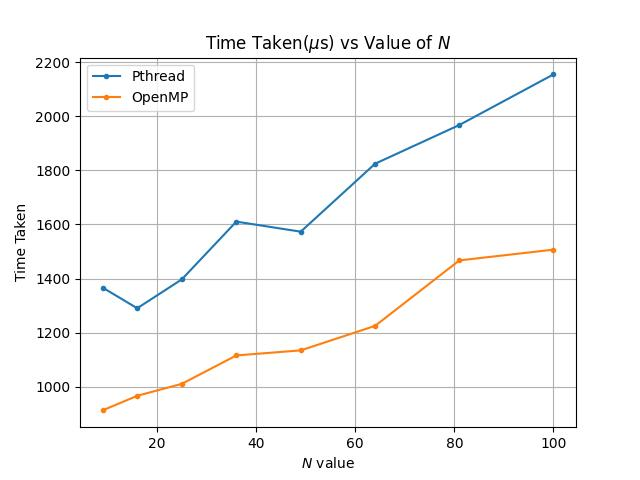
\includegraphics[width=1\textwidth]{plot_K_const}
		\caption{$T$ vs $N$ ($K$ is constant)}
	\end{figure}
	\subsubsection{Observations :}
	\begin{itemize}
		\item \underline{\textbf{Expected}} : As $N$ increases $T$ increases.
		\item \underline{\textbf{Observed}} : 
		\begin{itemize}
			\item The performance of OpenMP is better than Pthread.
			\item As expected the value of $T$ increases regularly in case of OpenMP on increasing $N$.
			\item In case of Pthread the graph looks to be increasing overally but there are small depressions at some values of $K$, this signifies that the peformace in case of those two threads is nearly same (as we are working with time in $\mu$s).
		\end{itemize}
		
	\end{itemize}
	\pagebreak
	\subsection{$N$ is constant :}
	\begin{itemize}
		\item The value of $N$ is fixed and is equal to $25$.
		\item Now we see the variation of time of excecuiton of program ($T$) by varying the total number of threads ($K$).
	\end{itemize}
	\subsubsection{Graph :}
	\begin{figure}[H]
		\centering
		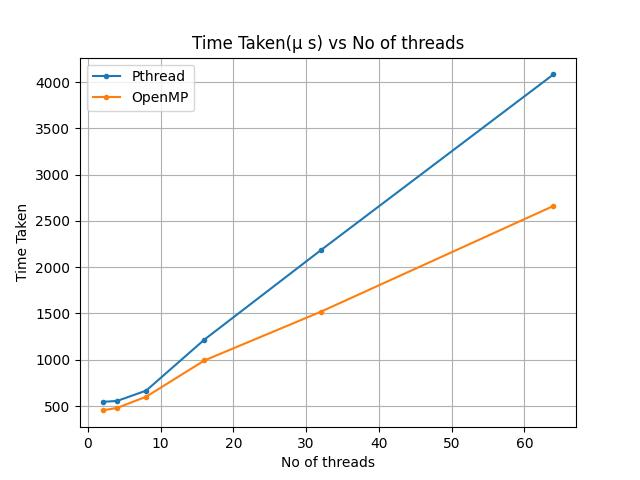
\includegraphics[width=1\textwidth]{plot_N_const}
		\caption{$T$ vs $K$ ($N$ is constant)}
	\end{figure}
	\subsubsection{Observations :} 
	\begin{itemize}
		\item \underline{\textbf{Expected}} : As $K$ increases $T$ decreases.
		\item \underline{\textbf{Observed}} : 
		\begin{itemize}
			\item  From the above graph we can conclude that OpenMP is faster than Pthreads.
			\item The value of time increases as $K$ increases because as the value of $N$ beign low.
			\item Generally threads work efficiently when we have a large amount of data, because in this context using threads makes sense, as splitting of work matters here.
			\item But when we have only less data doing the using threads is inefficient as at the first go there is no need of threading to be used.
			\item So here now as $N=25$, which is a low value and which doesn't need threading implementation.
			\item This is the reason why in this case as $K$ increases the execution time $T$ increases. 
		\end{itemize}
	\end{itemize}  		
		\section{ Final Conclusion:} 
		\begin{itemize}
			\item Using OpenMP we can do threading more fastly and efficiently than Pthreads.
		\end{itemize}
\end{document}



